\graphicspath{ {img/23/} }

\chapter{Nevýhody súčasných metód}
\section{Podpora mobilných zariadení}
\label{sec:mobile-support}

V roku 2010, Steve Jobs, spoluzakladateľ a~v tom čase aj výkonný riaditeľ Applu vydal vyhlásenie \emph{Thoughts on Flash} \cite{Apple_flash}, v~ktorom vysvetľuje, prečo zariadenia iPhone, iPod a~iPad nepodporujú \emph{Adobe Flash}. Kritizuje \emph{Adobe Flash} z~uzavretosti, vysokej systémovej záťaže, slabej bezpečnosti a~chýbajúcej podpory dotykových zariadení.
BBC v~roku 2012 informovala \cite{Android_flash}, že Adobe sťahuje \emph{Adobe Flash Player} z~\emph{Google Play Store}, čo dovtedy umožňovalo prehrávať \emph{Adobe Flash} na~mobilných zariadeniach. To znamená, že mobilné operačné systémy, ktoré dohromady zaberajú 96,7\% trhu \cite{Mobile_OS_share} nepodporujú \emph{Adobe Flash}.


\section{Zbytočné súbory na~serveri}

Nahrávanie obrázkov bez~toho, aby užívateľ najskôr obrázok videl, môže viesť k~tomu, že užívateľ nahrá nesprávny obrázok. Takisto môže vzniknúť problém, kedy užívateľ kvôli nesprávnemu spracovaniu obrázka na~serveri (napríklad nesprávny orez, pozri \ref{sec:orezanie-obrazka}), môže zmeniť svoje rozhodnutie. Takto vznikajú na~serveri súbory -- obrázky, ktoré sa nikdy nepoužijú. Jedno z~riešení tohto problému je pravidelné mazanie nevyužívaných obrázkov.   

\section{Orezanie obrázka}
\label{sec:orezanie-obrazka}

Pri spracovaní na~serveri zvyčajne dochádza k~zmenšeniu a~orezaniu obrázka. Spravidla sa obrázky orezávajú na~stred. To však môže byť nesprávne, ako ukazuje obrázok \ref{fig:jg_image}, kde orezanie na~stred odreže osobu -- najdôležitejšiu časť obrázka. Čiastočným riešením je využitie detekcie tvárí. Pokročilé riešenia si však vyžadujú pokročilú analýzu obrazu, kde sa analyzuje kontrast a~hrany. Vďaka tomu je možné detegovať východ slnka, alebo budovu na~obrázku. 

\begin{figure}[!ht]
	\centering
	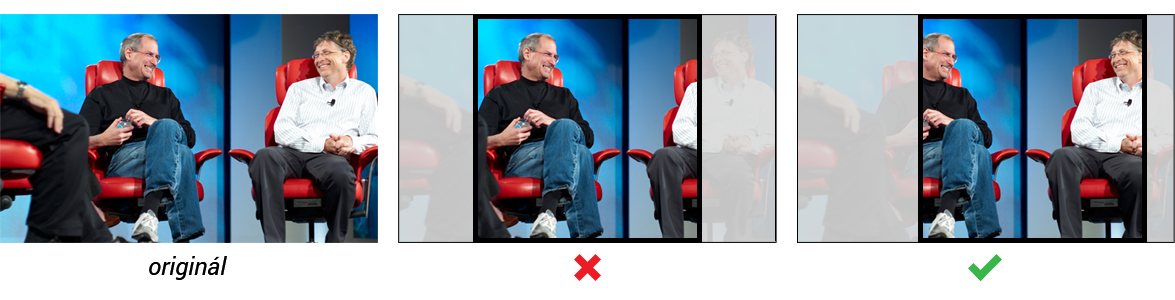
\includegraphics[width=\textwidth]{jobs_gates}
	\caption{Demonštrácia zlého automatického orezania obrázka. Pôvodný obrázok z~\cite{Jobs_Gates_piture}.}
	\label{fig:jg_image}
\end{figure}

% TODO: Originál v~obrázku

\section{Prenášanie zbytočných dát}

Spracovanie obrázka obvykle prebieha na~serveri. To však znamená, že ak je žiadaný len zmenšený a~orezaný obrázok, tak väčšina dát, ktoré užívateľ preniesol, je zbytočná. Pokiaľ by zmenšenie a~orezanie obrázka prebiehalo v~prehliadači, tak sa prenesie menej dát, čo zrýchli nahrávanie obrázka na~webový server a~tiež ušetrí peniaze v~prípade spoplatnených mobilných dát.

%Pre ilustráciu, aký veľký rozdiel to môže byť uvádzame aj jednoduché porovnanie. V~čase písania tejto práce mal najväčšie zastúpenie medzi~telefónmi značky \emph{Apple} model \emph{iPhone 6} \cite{Mixpanel_iphones}. Ten má zadný fotoaparát s~rozlíšením 8 megapixelov \cite{iPhone_camera}. \emph{W3Counter} uvádza, že najpoužívanejšie rozlíšenie je $1366 \times 768$ pixelov. To je 1,05 megapixelov. Na~štvrtom mieste (najväčšie rozlíšenie spomedzi piatich najpoužívanejších) je $1366 \times 768$ 